\documentclass[11pt,a4paper]{report}
\usepackage[textwidth=37em,vmargin=30mm]{geometry}
\usepackage{calc,xunicode,amsmath,amssymb,paralist,enumitem,tabu,booktabs,datetime2,xeCJK,xeCJKfntef,listings}
\usepackage{tocloft,fancyhdr,tcolorbox,xcolor,graphicx,eso-pic,xltxtra,xelatexemoji}

\newcommand{\envyear}[0]{2025}
\newcommand{\envdatestr}[0]{2025-01-11}
\newcommand{\envfinaldir}[0]{webdb/2025/20250111/final}

\usepackage[hidelinks]{hyperref}
\hypersetup{
    colorlinks=false,
    pdfpagemode=FullScreen,
    pdftitle={Web Digest - \envdatestr}
}

\setlength{\cftbeforechapskip}{10pt}
\renewcommand{\cftchapfont}{\rmfamily\bfseries\large\raggedright}
\setlength{\cftbeforesecskip}{2pt}
\renewcommand{\cftsecfont}{\sffamily\small\raggedright}

\setdefaultleftmargin{2em}{2em}{1em}{1em}{1em}{1em}

\usepackage{xeCJK,xeCJKfntef}
\xeCJKsetup{PunctStyle=plain,RubberPunctSkip=false,CJKglue=\strut\hskip 0pt plus 0.1em minus 0.05em,CJKecglue=\strut\hskip 0.22em plus 0.2em}
\XeTeXlinebreaklocale "zh"
\XeTeXlinebreakskip = 0pt


\setmainfont{Brygada 1918}
\setromanfont{Brygada 1918}
\setsansfont{IBM Plex Sans}
\setmonofont{JetBrains Mono NL}
\setCJKmainfont{Noto Serif CJK SC}
\setCJKromanfont{Noto Serif CJK SC}
\setCJKsansfont{Noto Sans CJK SC}
\setCJKmonofont{Noto Sans CJK SC}

\setlength{\parindent}{0pt}
\setlength{\parskip}{8pt}
\linespread{1.15}

\lstset{
	basicstyle=\ttfamily\footnotesize,
	numbersep=5pt,
	backgroundcolor=\color{black!5},
	showspaces=false,
	showstringspaces=false,
	showtabs=false,
	tabsize=2,
	captionpos=b,
	breaklines=true,
	breakatwhitespace=true,
	breakautoindent=true,
	linewidth=\textwidth
}






\newcommand{\coverpic}[2]{
    % argv: itemurl, authorname
    Cover photo by #2~~(\href{#1}{#1})
}
\newcommand{\makeheader}[0]{
    \begin{titlepage}
        % \newgeometry{hmargin=15mm,tmargin=21mm,bmargin=12mm}
        \begin{center}
            
            \rmfamily\scshape
            \fontspec{BaskervilleF}
            \fontspec{Old Standard}
            \fontsize{59pt}{70pt}\selectfont
            WEB\hfill DIGEST
            
            \vfill
            % \vskip 30pt
            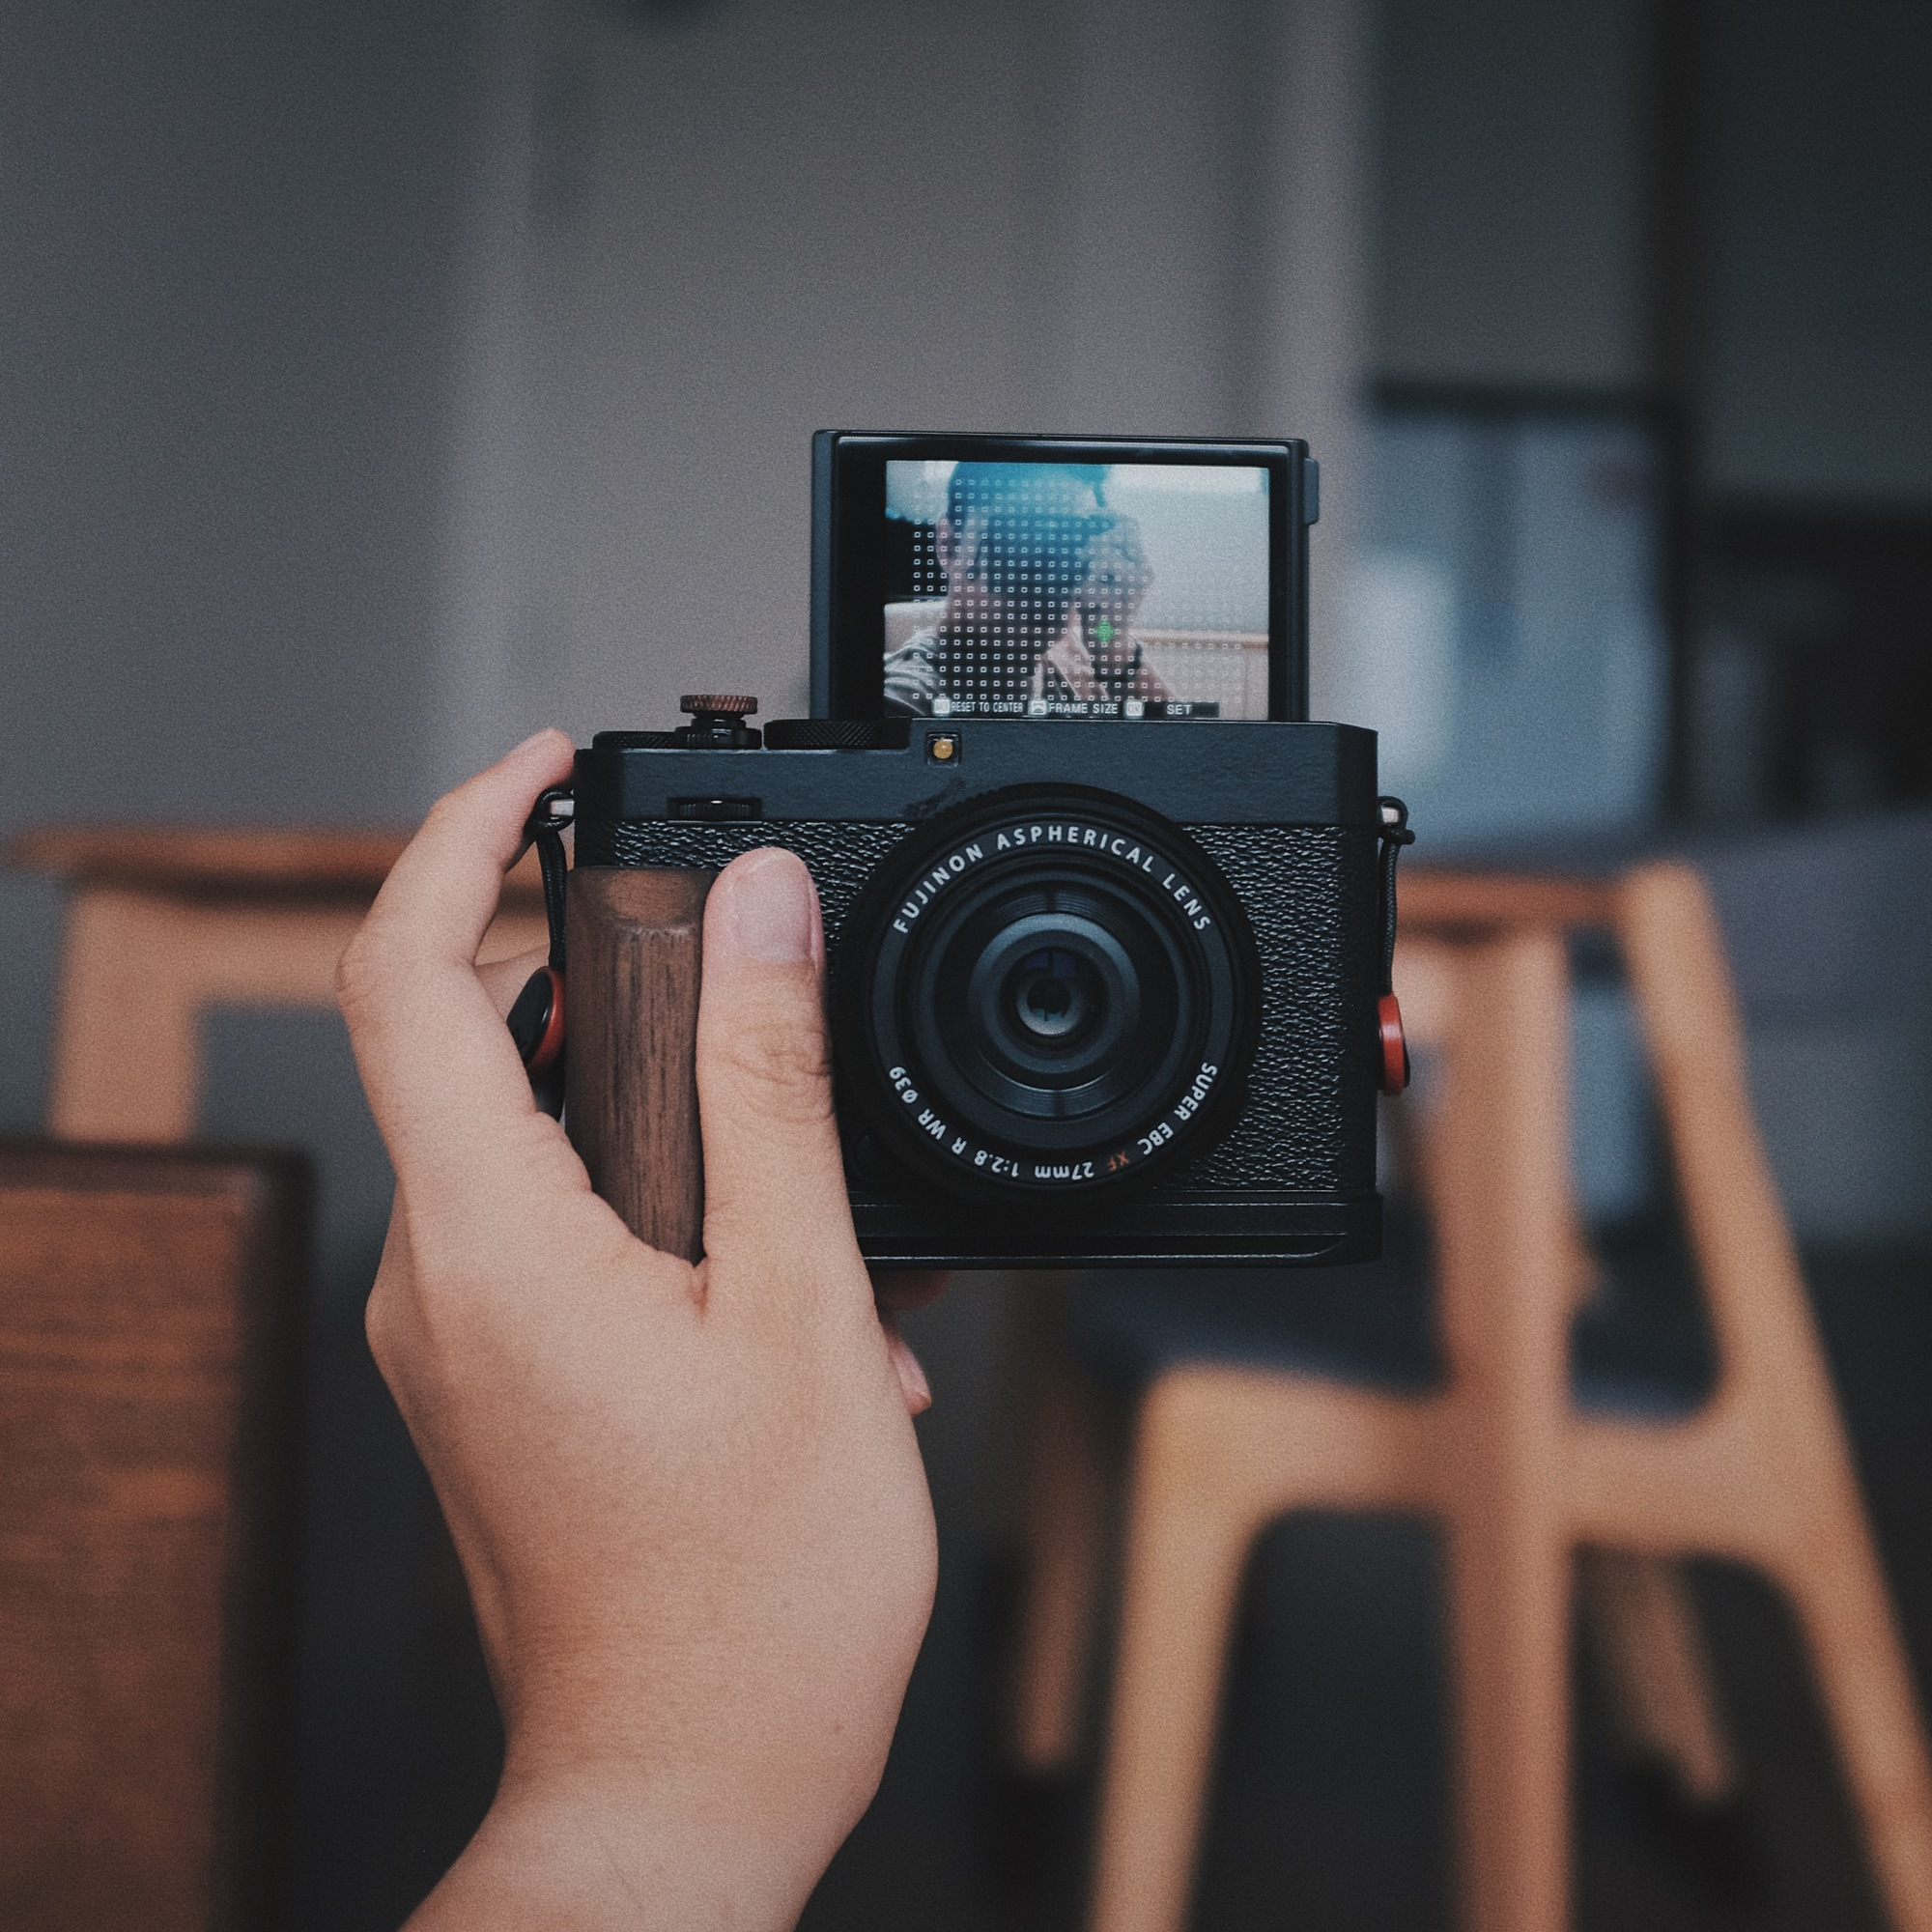
\includegraphics[width=\linewidth]{\envfinaldir/coverpic-prod.jpg}\par
            % \vskip 30pt
            \vfill

            \normalsize\rmfamily\scshape
            \copyright{} The Web Digest Project \hfill\large \envdatestr
        \end{center}
    \end{titlepage}
    % \restoregeometry
}
\newcommand{\simplehref}[1]{%
    \textcolor{blue!80!green}{\href{#1}{#1}}%
}
\renewcommand{\contentsname}{\center\Huge\sffamily\bfseries Contents\par\vskip 20pt}
\newcounter{ipartcounter}
\setcounter{ipartcounter}{0}
\newcommand{\ipart}[1]{
    % \vskip 20pt
    \clearpage
    \stepcounter{ipartcounter}
    \phantomsection
    \addcontentsline{toc}{chapter}{#1}
    % \begin{center}
    %     \Huge
    %     \sffamily\bfseries
    %     #1
    % \end{center}
    % \vskip 20pt plus 7pt
}
\newcounter{ichaptercounter}
\setcounter{ichaptercounter}{0}
\newcommand{\ichapter}[1]{
    % \vskip 20pt
    \clearpage
    \stepcounter{ichaptercounter}
    \phantomsection
    \addcontentsline{toc}{section}{\numberline{\arabic{ichaptercounter}}#1}
    \begin{center}
        \Huge
        \sffamily\bfseries
        #1
    \end{center}
    \vskip 20pt plus 7pt
}
\newcommand{\entrytitlefont}[1]{\subsection*{\raggedright\Large\sffamily\bfseries#1}}
\newcommand{\entryitemGeneric}[2]{
    % argv: title, url
    \parbox{\linewidth}{
        \entrytitlefont{#1}\par\vskip 5pt
        \footnotesize\ttfamily\mdseries
        \simplehref{#2}
    }\vskip 11pt plus 11pt minus 1pt
}
\newcommand{\entryitemGithub}[3]{
    % argv: title, url, desc
    \parbox{\linewidth}{
        \entrytitlefont{#1}\par\vskip 5pt
        \footnotesize\ttfamily\mdseries
        \simplehref{#2}\par\vskip 5pt
        \small\rmfamily\mdseries#3
    }\vskip 11pt plus 11pt minus 1pt
}
\newcommand{\entryitemAp}[3]{
    % argv: title, url, desc
    \parbox{\linewidth}{
        \entrytitlefont{#1}\par\vskip 5pt
        \footnotesize\ttfamily\mdseries
        \simplehref{#2}\par\vskip 5pt
        \small\rmfamily\mdseries#3
    }\vskip 11pt plus 11pt minus 1pt
}
\newcommand{\entryitemHackernews}[3]{
    % argv: title, hnurl, rawurl
    % \parbox{\linewidth}{
    %     \entrytitlefont{#1}\par\vskip 5pt
    %     \footnotesize\ttfamily\mdseries
    %     \simplehref{#3}\par
    %     \textcolor{black!50}{\href{#2}{#2}}
    % }\vskip 11pt plus 11pt minus 1pt
    \begin{minipage}{\linewidth}
            \entrytitlefont{#1}\par\vskip 5pt
            \footnotesize\ttfamily\mdseries
            \simplehref{#3}\par
            \textcolor{black!50}{\href{#2}{#2}}
    \end{minipage}\par\vskip 11pt plus 11pt minus 1pt
}







\begin{document}

\makeheader

\tableofcontents\clearpage




\ipart{Developers}
\ichapter{Hacker News}
\entryitemTwoLinks{Cuttle – a MTG like game using a standard 52 card deck}{https://news.ycombinator.com/item?id=42658614}{https://www.pagat.com/combat/cuttle.html}

\entryitemTwoLinks{Meta's memo to employees rolling back DEI programs}{https://news.ycombinator.com/item?id=42657901}{https://www.axios.com/2025/01/10/meta-dei-memo-employees-programs}

\entryitemTwoLinks{Starlink is now cheaper than leading internet provider in some African countries}{https://news.ycombinator.com/item?id=42657692}{https://restofworld.org/2025/starlink-cheaper-internet-africa/}

\entryitemTwoLinks{Getting silly with C, part (void*)2}{https://news.ycombinator.com/item?id=42657591}{https://lcamtuf.substack.com/p/getting-silly-with-c-part-void2}

\entryitemTwoLinks{Show HN: Freeact – A Lightweight Library for Code-Action Based Agents}{https://news.ycombinator.com/item?id=42657253}{https://github.com/gradion-ai/freeact}

\entryitemTwoLinks{Web apps built with Ruby on Rails}{https://news.ycombinator.com/item?id=42656559}{https://weuserails.com/}

\entryitemTwoLinks{Formal Methods: Just Good Engineering Practice? (2024)}{https://news.ycombinator.com/item?id=42656433}{https://brooker.co.za/blog/2024/04/17/formal}

\entryitemTwoLinks{I've acquired a new superpower}{https://news.ycombinator.com/item?id=42655870}{https://danielwirtz.com/blog/spot-the-difference-superpower}

\entryitemTwoLinks{The Tedious Heroism of David Ruggles}{https://news.ycombinator.com/item?id=42655636}{https://commonplace.online/article/the-tedious-heroism-of-david-ruggles/}

\entryitemTwoLinks{I got OpenTelemetry to work. But why was it so complicated?}{https://news.ycombinator.com/item?id=42655102}{https://iconsolutions.com/blog/i-got-opentelemetry-to-work-but-why-was-it-so-complicated/}

\entryitemTwoLinks{Learning How to Think with Meta Chain-of-Thought}{https://news.ycombinator.com/item?id=42655098}{https://arxiv.org/abs/2501.04682}

\entryitemTwoLinks{Who Can Understand the Proof? A Window on Formalized Mathematics}{https://news.ycombinator.com/item?id=42654995}{https://writings.stephenwolfram.com/2025/01/who-can-understand-the-proof-a-window-on-formalized-mathematics/}

\entryitemTwoLinks{Nvidia-Ingest: Multi-modal data extraction}{https://news.ycombinator.com/item?id=42654019}{https://github.com/NVIDIA/nv-ingest}

\entryitemTwoLinks{Glimmer: DSL Framework for Ruby GUI and More}{https://news.ycombinator.com/item?id=42653939}{https://github.com/AndyObtiva/glimmer}

\entryitemTwoLinks{Tactility: OS for the ESP32 Microcontroller Family}{https://news.ycombinator.com/item?id=42653811}{https://tactility.one/\#/}

\entryitemTwoLinks{Before Squid Game, there was Battle Royale}{https://news.ycombinator.com/item?id=42652967}{https://www.tokyoweekender.com/entertainment/movies-tv/before-squid-game-there-was-battle-royale/}

\entryitemTwoLinks{Visualizing All ISBNs}{https://news.ycombinator.com/item?id=42652577}{https://annas-archive.org/blog/all-isbns.html}

\entryitemTwoLinks{Gleam v1.7}{https://news.ycombinator.com/item?id=42652329}{https://gleam.run/news/improved-performance-and-publishing/}

\entryitemTwoLinks{A three month review of kagi search and the orion web browser (2024)}{https://news.ycombinator.com/item?id=42652125}{https://flatfootfox.com/a-three-month-review-of-kagi-search-the-orion-web-browser/}

\entryitemTwoLinks{41\% of Employers Worldwide Say They'll Reduce Staff by 2030 Due to AI}{https://news.ycombinator.com/item?id=42652076}{https://gizmodo.com/41-of-employers-worldwide-say-theyll-reduce-staff-by-2030-due-to-ai-2000548131}\ichapter{Phoronix}
\entryitemGeneric{\hskip 0pt{}Wine 10.0-rc5 Brings Another 31 Bug Fixes}{https://www.phoronix.com/news/Wine-10.0-rc5}

\entryitemGeneric{\hskip 0pt{}Experimental Linux Address Space Isolation "ASI" v2 Patches: I/O Throughput Lower By 70\%}{https://www.phoronix.com/news/Google-Linux-ASI-v2-RFC-Patches}

\entryitemGeneric{\hskip 0pt{}Git 2.48 Released With Initial Support For The Meson Build System}{https://www.phoronix.com/news/Git-2.48-Released}

\entryitemGeneric{\hskip 0pt{}More Intel Xeon Clearwater Forest Enablement Merged For Linux 6.13}{https://www.phoronix.com/news/Linux-6.13-More-Intel-CWF}

\entryitemGeneric{\hskip 0pt{}Lenovo Discovers Situation Of Linux Dropping PCIe Gen 5 NVMe SSDs To Gen 1 Speeds}{https://www.phoronix.com/news/Lenovo-Linux-NVMe-Gen5-To-Gen1}

\entryitemGeneric{\hskip 0pt{}Servo Browser Engine Adds Dark Mode, Some XPath Support}{https://www.phoronix.com/news/Servo-December-2024}

\entryitemGeneric{\hskip 0pt{}VKD3D-Proton 2.14.1 Brings A Few Fixes For Direct3D 12 On Vulkan}{https://www.phoronix.com/news/VKD3D-Proton-2.14.1-Released}

\entryitemGeneric{\hskip 0pt{}Ubuntu Considers Taking It Easier On Software Updates Over Weekends}{https://www.phoronix.com/news/Ubuntu-Considers-Light-Weekends}

\entryitemGeneric{\hskip 0pt{}12 Years After Haswell, Intel Open-Source Graphics Developers Still Make Occasional Fix}{https://www.phoronix.com/news/Haswell-Engine-Fix-For-Linux-25}\ichapter{Dribbble}
\entryitemGeneric{\hskip 0pt{}SHOWREEL 24'}{https://dribbble.com/shots/25450148-SHOWREEL-24}

\entryitemGeneric{\hskip 0pt{}Business set}{https://dribbble.com/shots/25444987-Business-set}

\entryitemGeneric{\hskip 0pt{}Pageless Logo \& Visual Identity}{https://dribbble.com/shots/25450527-Pageless-Logo-Visual-Identity}

\entryitemGeneric{\hskip 0pt{}Cromatic.bio®}{https://dribbble.com/shots/25451539-Cromatic-bio}

\entryitemGeneric{\hskip 0pt{}Running Dog Logo}{https://dribbble.com/shots/25450403-Running-Dog-Logo}

\entryitemGeneric{\hskip 0pt{}B}{https://dribbble.com/shots/25449124-B}

\entryitemGeneric{\hskip 0pt{}Tempest Logo Design \& Visual Identity}{https://dribbble.com/shots/25371917-Tempest-Logo-Design-Visual-Identity}

\entryitemGeneric{\hskip 0pt{}HR Management Dashboard}{https://dribbble.com/shots/25442919-HR-Management-Dashboard}

\entryitemGeneric{\hskip 0pt{}Milky Giant Studios Logo}{https://dribbble.com/shots/25403425-Milky-Giant-Studios-Logo}

\entryitemGeneric{\hskip 0pt{}Cute Chicken Logo}{https://dribbble.com/shots/25443854-Cute-Chicken-Logo}

\entryitemGeneric{\hskip 0pt{}Bexet}{https://dribbble.com/shots/25440591-Bexet}

\entryitemGeneric{\hskip 0pt{}Down the drain}{https://dribbble.com/shots/25445263-Down-the-drain}

\entryitemGeneric{\hskip 0pt{}Love}{https://dribbble.com/shots/25446955-Love}

\entryitemGeneric{\hskip 0pt{}Placefully - Logo Design}{https://dribbble.com/shots/25437901-Placefully-Logo-Design}

\entryitemGeneric{\hskip 0pt{}Portex}{https://dribbble.com/shots/25434801-Portex}

\entryitemGeneric{\hskip 0pt{}Every Cast Counts!™}{https://dribbble.com/shots/25439476-Every-Cast-Counts}

\entryitemGeneric{\hskip 0pt{}Vox - Brandmark}{https://dribbble.com/shots/25429765-Vox-Brandmark}

\entryitemGeneric{\hskip 0pt{}Dropbox - Logo Redesign}{https://dribbble.com/shots/25432726-Dropbox-Logo-Redesign}

\entryitemGeneric{\hskip 0pt{}Logo Design 2 for Ai Assistant (Unused for Sale)}{https://dribbble.com/shots/25433244-Logo-Design-2-for-Ai-Assistant-Unused-for-Sale}

\entryitemGeneric{\hskip 0pt{}Behemoths}{https://dribbble.com/shots/25433176-Behemoths}

\entryitemGeneric{\hskip 0pt{}Run it back}{https://dribbble.com/shots/25430165-Run-it-back}

\entryitemGeneric{\hskip 0pt{}Alder Posters}{https://dribbble.com/shots/25433543-Alder-Posters}

\entryitemGeneric{\hskip 0pt{}Attio homepage redesign}{https://dribbble.com/shots/25432766-Attio-homepage-redesign}

\entryitemGeneric{\hskip 0pt{}Hooke Outdoor Co.}{https://dribbble.com/shots/25429227-Hooke-Outdoor-Co}


\ipart{Developers~~~~(zh-Hans)}
\ichapter{Solidot}
\entryitemGeneric{\hskip 0pt{}独立分析认为巴勒斯坦卫生部严重低估了加沙死亡人数}{https://www.solidot.org/story?sid=80300}

\entryitemGeneric{\hskip 0pt{}四分之一淡水动物面临灭绝}{https://www.solidot.org/story?sid=80299}

\entryitemGeneric{\hskip 0pt{}美国司法部准备出售扣押的丝绸之路比特币}{https://www.solidot.org/story?sid=80298}

\entryitemGeneric{\hskip 0pt{}法官拒绝了试图从垃圾堆里挖出 8000 比特币的诉讼}{https://www.solidot.org/story?sid=80297}

\entryitemGeneric{\hskip 0pt{}三星量产笔记本用的卷轴 OLED 显示屏}{https://www.solidot.org/story?sid=80296}

\entryitemGeneric{\hskip 0pt{}2024 年是平均气温比工业化前水平高出1.5 摄氏度的第一年}{https://www.solidot.org/story?sid=80295}

\entryitemGeneric{\hskip 0pt{}氟化物暴露与 IQ 分数低相关}{https://www.solidot.org/story?sid=80294}

\entryitemGeneric{\hskip 0pt{}中国在前沿 AI 研究上紧追美国}{https://www.solidot.org/story?sid=80293}

\entryitemGeneric{\hskip 0pt{}中国风投让失败的创业者成为失信债务人}{https://www.solidot.org/story?sid=80292}

\entryitemGeneric{\hskip 0pt{}ispace 准备再次发射登月舱}{https://www.solidot.org/story?sid=80291}

\entryitemGeneric{\hskip 0pt{}乳腺癌是最常见的癌症肺癌是最致命的癌症}{https://www.solidot.org/story?sid=80290}

\entryitemGeneric{\hskip 0pt{}拜登计划在离任前对 AI 芯片出口实施新限制}{https://www.solidot.org/story?sid=80289}

\entryitemGeneric{\hskip 0pt{}VLC 预览本地 AI 字幕翻译功能}{https://www.solidot.org/story?sid=80288}

\entryitemGeneric{\hskip 0pt{}WHO 称中国的人偏肺病毒感染在正常水平}{https://www.solidot.org/story?sid=80287}

\entryitemGeneric{\hskip 0pt{}Google 为停止支持的 Pixel 4a 释出新更新,代价是电池寿命缩短}{https://www.solidot.org/story?sid=80286}

\entryitemGeneric{\hskip 0pt{}树莓派推出售价 120 美元 16GB 内存版本的 Raspberry Pi 5}{https://www.solidot.org/story?sid=80285}

\entryitemGeneric{\hskip 0pt{}眨眼可能有助于认知休息}{https://www.solidot.org/story?sid=80284}

\entryitemGeneric{\hskip 0pt{}Firefox 134.0 释出}{https://www.solidot.org/story?sid=80283}

\entryitemGeneric{\hskip 0pt{}日本警告中国黑客攻击}{https://www.solidot.org/story?sid=80282}

\entryitemGeneric{\hskip 0pt{}Telegram 向美国提供了数千用户数据}{https://www.solidot.org/story?sid=80281}\ichapter{V2EX}
\entryitemGeneric{\hskip 0pt{}[问与答] 请问 next.js 里如何好好渲染 md}{https://www.v2ex.com/t/1104302}

\entryitemGeneric{\hskip 0pt{}[问与答] 有没有哪家国产手机支持类似三星 Dex 的功能}{https://www.v2ex.com/t/1104301}

\entryitemGeneric{\hskip 0pt{}[信息安全] 现在 SHA1 已经属于不安全的 hash 算法了,但是很多软件的 codesign 还是 SHA1 的,是否有伪造签名的风险?}{https://www.v2ex.com/t/1104300}

\entryitemGeneric{\hskip 0pt{}[美国] 最高法院听取关于 TikTok 禁令的案件。2025 年 1 月 10 日。暗示可能会维持美国的 TikTok 禁令}{https://www.v2ex.com/t/1104299}

\entryitemGeneric{\hskip 0pt{}[程序员] 使用 Canvas 模拟键盘音乐律动效果}{https://www.v2ex.com/t/1104297}

\entryitemGeneric{\hskip 0pt{}[SSH] mosh ssh 问题}{https://www.v2ex.com/t/1104296}

\entryitemGeneric{\hskip 0pt{}[问与答] 如何把项目代码全部提交给 AI 进行阅读呢}{https://www.v2ex.com/t/1104295}

\entryitemGeneric{\hskip 0pt{}[问与答] 想开发全平台带 UGC 的 App,现在需要哪些资质?}{https://www.v2ex.com/t/1104294}

\entryitemGeneric{\hskip 0pt{}[分享创造] 做了一个 SmolAgent 的介绍和教程网站,不知道大家有什么建议没?}{https://www.v2ex.com/t/1104292}

\entryitemGeneric{\hskip 0pt{}[推广] 一个稳定的 chatgpt 接口 、midjourney 接口、suno 接口平台}{https://www.v2ex.com/t/1104288}

\entryitemGeneric{\hskip 0pt{}[问与答] AI 时代,纠结还要不要深入学 Java}{https://www.v2ex.com/t/1104287}

\entryitemGeneric{\hskip 0pt{}[分享发现] 苹果官方红包封面}{https://www.v2ex.com/t/1104286}

\entryitemGeneric{\hskip 0pt{}[问与答] 有懂音箱的吗?最近想入 sonos Era 300}{https://www.v2ex.com/t/1104285}

\entryitemGeneric{\hskip 0pt{}[Apple] 有没有不贵的摄像头 onvif 客户端? mac 与 iPhone 平台}{https://www.v2ex.com/t/1104279}

\entryitemGeneric{\hskip 0pt{}[问与答] 求问各位 V 友,有那些 API 资源管理服务?}{https://www.v2ex.com/t/1104277}

\entryitemGeneric{\hskip 0pt{}[Python] Flask+SQLite+Tornado 在 Windows 2019 下 100 并发都撑不住是怎么回事?}{https://www.v2ex.com/t/1104276}

\entryitemGeneric{\hskip 0pt{}[职场话题] 大部分公司春节都是提前一周放假的吗}{https://www.v2ex.com/t/1104274}

\entryitemGeneric{\hskip 0pt{}[问与答] Gemini API 的 token 到底是怎么计的?}{https://www.v2ex.com/t/1104273}

\entryitemGeneric{\hskip 0pt{}[分享创造] 一个比较科学的穿衣计算器}{https://www.v2ex.com/t/1104272}

\entryitemGeneric{\hskip 0pt{}[问与答] 开发的软件如何优雅的同时适配 win 和 macos}{https://www.v2ex.com/t/1104271}

\entryitemGeneric{\hskip 0pt{}[分享创造] 你们日常是怎么提升自己的心力的}{https://www.v2ex.com/t/1104269}

\entryitemGeneric{\hskip 0pt{}[酷工作] [招聘] [远程办公] Ai Agent 产品经理}{https://www.v2ex.com/t/1104267}

\entryitemGeneric{\hskip 0pt{}[Local LLM] 我做了一个 Ollama 模型仓库镜像站,帮你更快的从 ModelScope 魔搭拉取模型}{https://www.v2ex.com/t/1104266}

\entryitemGeneric{\hskip 0pt{}[生活] 不想做女友的情绪垃圾桶是我的错吗?}{https://www.v2ex.com/t/1104265}

\entryitemGeneric{\hskip 0pt{}[宽带症候群] 北京联通如何跑 PT 不被限制上传}{https://www.v2ex.com/t/1104264}

\entryitemGeneric{\hskip 0pt{}[问与答] 把 openai 或 deepseek 的 api key 写到 GUI 客户端里会被网络抓包软件嗅探到吗?}{https://www.v2ex.com/t/1104262}

\entryitemGeneric{\hskip 0pt{}[问与答] 连接奥睿科的硬盘盒到他家的 usb hub 会导致硬盘访问异常, 包括无法识别硬盘、访问中断、识别很慢、读写很慢.}{https://www.v2ex.com/t/1104258}

\entryitemGeneric{\hskip 0pt{}[问与答] 为什么闲鱼外版 iPhone 没有发票?}{https://www.v2ex.com/t/1104257}

\entryitemGeneric{\hskip 0pt{}[游戏] 求推荐 FPS 耳机}{https://www.v2ex.com/t/1104256}

\entryitemGeneric{\hskip 0pt{}[问与答] 怎么买到合适的摩托车?}{https://www.v2ex.com/t/1104255}

\entryitemGeneric{\hskip 0pt{}[VPS] 阿里云学生认证的 300 元券机制是不是改了}{https://www.v2ex.com/t/1104252}

\entryitemGeneric{\hskip 0pt{}[问与答] 大佬们用 poe 提取的 token 处理东西感觉贵么}{https://www.v2ex.com/t/1104251}

\entryitemGeneric{\hskip 0pt{}[问与答] (2025 年 1 月)安卓手机与 iPhone 如何双向同步联系人?}{https://www.v2ex.com/t/1104249}

\entryitemGeneric{\hskip 0pt{}[问与答] 安卓的 apk 不上架到各大应用市场是不是也都可以被简单地用浏览器在线安装?}{https://www.v2ex.com/t/1104247}

\entryitemGeneric{\hskip 0pt{}[Visual Studio Code] 遇到一个关于设置中 auto Repository Detection(自动检测仓库)的 bug}{https://www.v2ex.com/t/1104245}

\entryitemGeneric{\hskip 0pt{}[酷工作] No AI without APIs, Kong 中国现开放 21 个技术岗位,期待你的加入!}{https://www.v2ex.com/t/1104244}

\entryitemGeneric{\hskip 0pt{}[OpenAI] deepseek v3/ qwen plus 都失败的编程题}{https://www.v2ex.com/t/1104243}

\entryitemGeneric{\hskip 0pt{}[北京] 北京回龙观 上北鑫座小区 49 平开间 业主直租 4000/每月}{https://www.v2ex.com/t/1104242}

\entryitemGeneric{\hskip 0pt{}[反馈] 为啥我没法发帖了?}{https://www.v2ex.com/t/1104241}

\entryitemGeneric{\hskip 0pt{}[Android] 有同学搞过安卓密钥过期的解决方案吗?}{https://www.v2ex.com/t/1104240}

\entryitemGeneric{\hskip 0pt{}[NAS] 馒头保种,怎么批量导入很多}{https://www.v2ex.com/t/1104239}

\entryitemGeneric{\hskip 0pt{}[宽带症候群] 福建联通家宽开始流量限制}{https://www.v2ex.com/t/1104238}

\entryitemGeneric{\hskip 0pt{}[Apple] Apple ID 迁移 10 个月依旧卡在云上贵州}{https://www.v2ex.com/t/1104237}

\entryitemGeneric{\hskip 0pt{}[酷工作] [全职远程] 英国伦敦二游公司直招 unity 开发工程师}{https://www.v2ex.com/t/1104235}

\entryitemGeneric{\hskip 0pt{}[美酒与美食] 吐槽一下现在在麦当劳汉堡王之类的快餐店很难喝到现打带汽的可乐}{https://www.v2ex.com/t/1104233}

\entryitemGeneric{\hskip 0pt{}[Apple] Mac mini M4 每天都会跟妙控键鼠断连一两次}{https://www.v2ex.com/t/1104232}

\entryitemGeneric{\hskip 0pt{}[程序员] 求教,最近写了一段时间 C\# WPF, 仅从写样式角度,感觉比起 HTML/CSS 非常麻烦,纯 windows 桌面应用 C\#下有其他更好用的框架吗?}{https://www.v2ex.com/t/1104231}

\entryitemGeneric{\hskip 0pt{}[问与答] RustDesk 移动端如何切换键盘模式?}{https://www.v2ex.com/t/1104230}

\entryitemGeneric{\hskip 0pt{}[分享发现] Vooh - 可能是最接近原生 iOS App 的 PWA}{https://www.v2ex.com/t/1104229}

\entryitemGeneric{\hskip 0pt{}[Apple] 苹果开发者注册遇到问题 有没有过来人可以支招}{https://www.v2ex.com/t/1104228}


\ipart{Generic News}







\clearpage
\leavevmode\vfill
\footnotesize

Copyright \copyright{} 2023-2025 Neruthes and other contributors.

This document is published with CC BY-NC-ND 4.0 license.

The entries listed in this newsletter may be copyrighted by their respective creators.

This newsletter is generated by the Web Digest project.

The newsletters are also delivered via Telegram channel \CJKunderline{\href{https://t.me/webdigestchannel}{https://t.me/webdigestchannel}}.\\
RSS feed is available at \CJKunderline{\href{https://webdigest.pages.dev/rss.xml}{https://webdigest.pages.dev/rss.xml}}.

This newsletter is available in PDF at
\CJKunderline{\href{https://webdigest.pages.dev/}{https://webdigest.pages.dev/}}.

The source code being used to generate this newsletter is available at\\
\CJKunderline{\href{https://github.com/neruthes/webdigest}{https://github.com/neruthes/webdigest}}.

This newsletter is also available in
\CJKunderline{\href{http://webdigest.pages.dev/readhtml/\envyear/WebDigest-20250111.html}{HTML}} and
\CJKunderline{\href{https://github.com/neruthes/webdigest/blob/master/markdown/\envyear/WebDigest-20250111.md}{Markdown}}.


\coverpic{https://unsplash.com/photos/a-view-of-a-waterfall-from-a-high-point-of-view-LuiP3ojMg5w}{Spenser Sembrat}


\end{document}
